\subsection{\emph{uOS}}
\label{subsec:introUos}

O \emph{middleware} \emph{uOS} é o resultado do projeto \emph{UbiquitOS} da Universidade de Brasília, cujo foco está na adaptabilidade de serviços. Nesse projeto, os dispositivos presentes em um ambiente inteligente são compostos por recursos que disponibilizam diversos serviços para aplicações ou para o próprio usuário final. Foi concebido um protocolo próprio para comunicação, o \emph{uP (Ubiquitous Protocols)} que utiliza o SLP (\emph{Service Location Protocol}) como técnica para descoberta de dispositivos e \emph{JSON} como formato para troca de mensagens.

\begin{figure}[ht]
	\center
	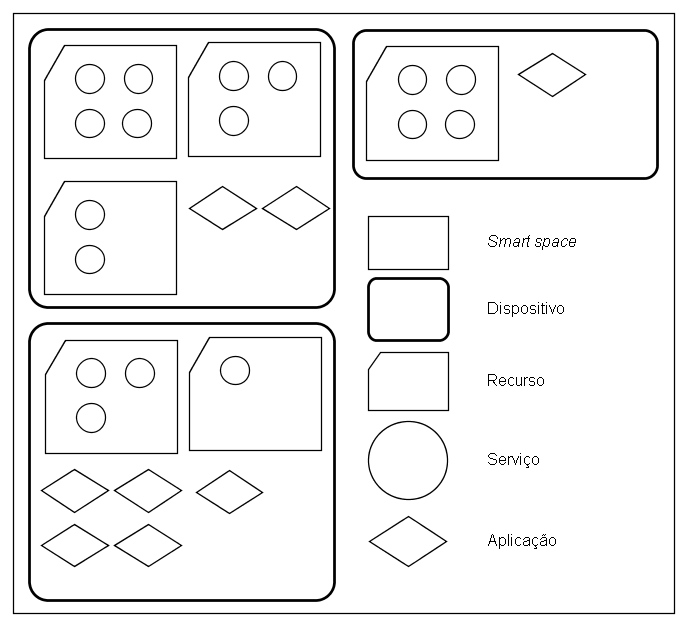
\includegraphics[scale=0.6]{imagens/arquiteturaDSOA}
	\caption{Exemplo da arquitetura DSOA.}
	\label{fig:arquiteturaDSOA}
\end{figure}

O \emph{uOS} utiliza a \emph{DSOA (Device Service Oriented Architecture)}~\cite{buzetoDSOA2010}, uma extensão da \emph{SOA (Service Oriented Architecure)}, como arquitetura. Como mostrado pela Figura~\ref{fig:arquiteturaDSOA}, na DSOA podemos destacar cinco entidades básicas: ambiente inteligente, dispositivo, recurso, serviço e aplicações. O ambiente inteligente é um espaço composto por pelo menos dois dispositivos com capacidade de computação conectados por meio de uma rede de comunicação com os usuários. Um dispositivo é definido como um aparelho com capacidade de comunicação e que pode abrigar aplicações. Um recurso é definido como um grupo de funcionalidades relacionadas que podem ser acessadas por meio de interfaces pré-definidas e é considerada a entidade básica de interação entre dispositivos. Um serviço é a implementação de uma funcionalidade disponibilizada pelo recurso para o ambiente com uma interface conhecida. As aplicações conferem inteligência ao ambiente executando nos dispositivos existentes e, a partir de informações providas pelos recursos conhecidos, podem realizar ações. 

Segundo a DSOA, cada recurso, modelado na forma de um \emph{driver}, é identificado por um nome e não há qualquer tipo de relacionamento entre outros recursos. A \emph{DSOA} não define tipos básicos de recursos.	

\begin{figure}[ht]
	\center
	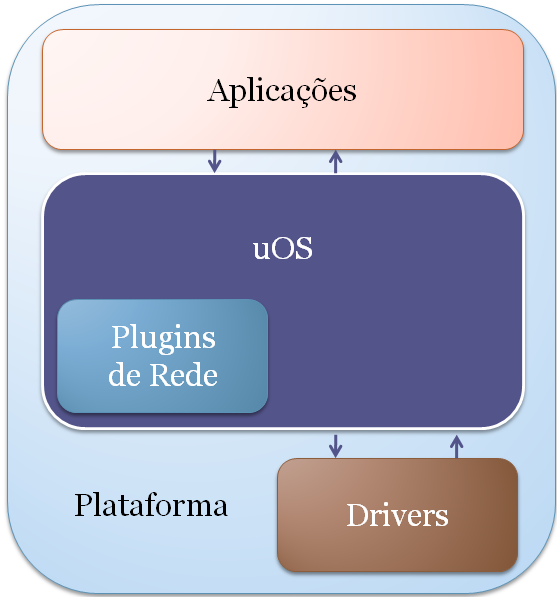
\includegraphics[scale=0.4]{imagens/ecossistemaUbiquitos}
	\caption{Ecossistema do \emph{uOS}.}
	\label{fig:ecossistemaUbiquitos}
\end{figure}

A Figura~\ref{fig:ecossistemaUbiquitos} mostra o ecossistema do \emph{uOS}, em que os \emph{plugins} de rede, abstrações para a rede de comunicação, se destacam como um componente dentro do \emph{uOS}. O \emph{middleware}, por sua vez, utiliza os \emph{plugins} para interfacear a comunicação entre aplicações, por meio dos \emph{drivers}.